\begin{refsection}[research/hori/group.bib]
\nocite{*}
\chapter{Computational Disaster Mitigation and Reduction Research Unit}

%.....................................................................
\section{Members}

\begin{itemize}
  \item[] Muneo Hori (Unit Leader)
  \item[] Hideyuki Ohtani (Research Scientist)
  \item[] Jian Chen (Research Scientist)
  \item[] Kohei Fujita (Research Scientist)
\end{itemize}

%.....................................................................
\section{Research Activities}

Computational disaster mitigation and reduction research unit is aimed at developing advanced large-scale numerical simulation of natural disasters such as an earthquake, tsunami and heavy rain, for Kobe City and other urban areas in Hyogo Prefecture. Besides for the construction of a sophisticated urban area model and the development of new numerical codes, the unit seeks to be a bridge between Science and Local Government for the disaster mitigation and reduction. 

Our research unit addressed the following research objects in this fiscal year:

\noindent
1) Construction of next generation hazard map for Kobe City. For two scenarios of Nankai Trough Earthquake presumed by National Government, the unit constructed next generation hazard map for Kobe City. Unlike conventional hazard map, the next generation hazard map is based on large scale numerical simulation of the physical processes of seismic wave propagation and seismic structural responses. The map achieves highest spatial resolution as well as higher rationality. Urban area models of Kobe City for underground and man-made structures are used in the physical simulation, and it is these models that determine the quality of the simulation; a more accurate model makes a more reliable estimation of earthquake hazard and disaster. Computational Disaster Mitigation and Reduction Research Unit develops a system that automatically constructs the urban area models using available data resources such as commercial Geographical Information System and governmental data. The system is designed to have high flexibility and expandability so that it can be used for various urban area to which suitable data resources are available.

\noindent
2) Development of system for liquefaction occurrence estimation. Due to complicated processes, the liquefaction occurrence ought to be estimated by using empirical equations that use engineering indices of soil layers of a target site. Computational Disaster Mitigation and Reduction Research Unit constructs a system that estimates the liquefaction occurrence using numerical simulation of the processes of liquefaction, i.e. coupling of soil deformation and underground water flow induced by ground motion. The system succeeds to automatically generate an underground model for 10,000 sites in Kobe City using available boring data and to simultaneously estimate the liquefaction occurrence for a measured or presumed ground motion.

\noindent
3) Estimation of lifeline damage induced by earthquake. Lifeline, or a network of buried pipelines of energy, water and communication, is an essential part of an urban area. Lifeline is damaged by ground deformation or strain, rather than ground motion such as acceleration or velocity, and hence three-dimensional analysis of underground structure responses for a given earthquake is needed to estimate lifeline damage induced by an earthquake. Using large scale finite element method, Computational Disaster Mitigation and Reduction Research Unit is developing a system that estimate lifeline damage, numerically simulating ground deformation of a target area.

%.....................................................................
\section{Research Results and Achievements}

%.....................................................................
\subsection{Construction of next generation hazard map for Kobe City}

National Government has studied a possible scenario of Nankai Trough Earthquake. Two large and extremely large scenarios have been announced for preparation of earthquake disaster. A distribution of possible ground motion index (such as seismic index or peak ground acceleration/velocity) and residential building damage is reported; this distribution is computed by using conventional method of empirical equations. The distribution is summarized as a hazard map for relatively large "mesh" or "grid" of more than 500 m or town-wise number of damaged houses.

Computational Disaster Mitigation and Reduction Research Unit constructs next generation hazard map for Kobe City, using the two presumed scenarios of National Government; see Fig.~\localref{hori:fig:hazard_map}. Unlike the conventional hazard map, the next generation hazard map takes advanage of large scale numerical simulation of the two physical processes, namely, the seismic wave propagation/amplification and the seismic structural responses. Numerical analysis methods for the physical processes are tuned for K computer, and the unit develops underground models for the seismic wave propagation/amplification process and a set of residential buildings the number of which exceeds 100,000 for Kobe City.

%.....................................................................
\begin{figure}
\centering
\includegraphics[scale=0.5]{research/hori/figure/hazard_map.eps}
\caption{Example of next generation hazard map for Kobe City}
\locallabel{hori:fig:hazard_map}
\end{figure}
%.....................................................................

The next generation hazard map has much higher spatial resolution of possible earthquake hazard and damage; for instance, the next generation hazard map is able to compute the seismic response of a residential house by inputting ground motion of the building's site. The map is more rational than the hazard map since it is based on the simulation of the physical processes. Many ground motions could share the same ground motion index, but they surely produce different seismic response for various structures. This is a reason why the simulation of the physical processes of the seismic wave propagation/amplification and the seismic structural responses is made for seismic design.

We have to mention that while the next generation hazard map has higher spatial resolution and rationality, it is the urban model that determines the quality of the hazard map. That is, a more accurate urban model of underground and man-made structures makes a more reliable estimation of earthquake hazard and disaster. The data that are used to construct the urban are model has limited quality and quantity, and hence the models are not perfect. A possible range of earthquake hazard and damage could be estimated by ensemble simulation that uses a numerous set of urban area models which are randomly generated in view of the uncertainty of the data.

The automated construction of an urban area model is a key element of the next generation hazard map. Computational Disaster Mitigation and Reduction Research Unit develops a system that automatically constructs the urban area models, making use of all available data resources such as commercial Geographical Information System and governmental data managed by various sections of local government; see Fig.~\localref{hori:fig:platform}. The system is designed to have high flexibility and expandability, as it takes full advantage of object oriented and aspect oriented programming; the use of aspect oriented programming is especially important since the system has to deal with data of similar data structures but distinct attributes. Hence, is can be used for other urban areas to which suitable data resources are available.

%.....................................................................
\begin{figure}
\centering
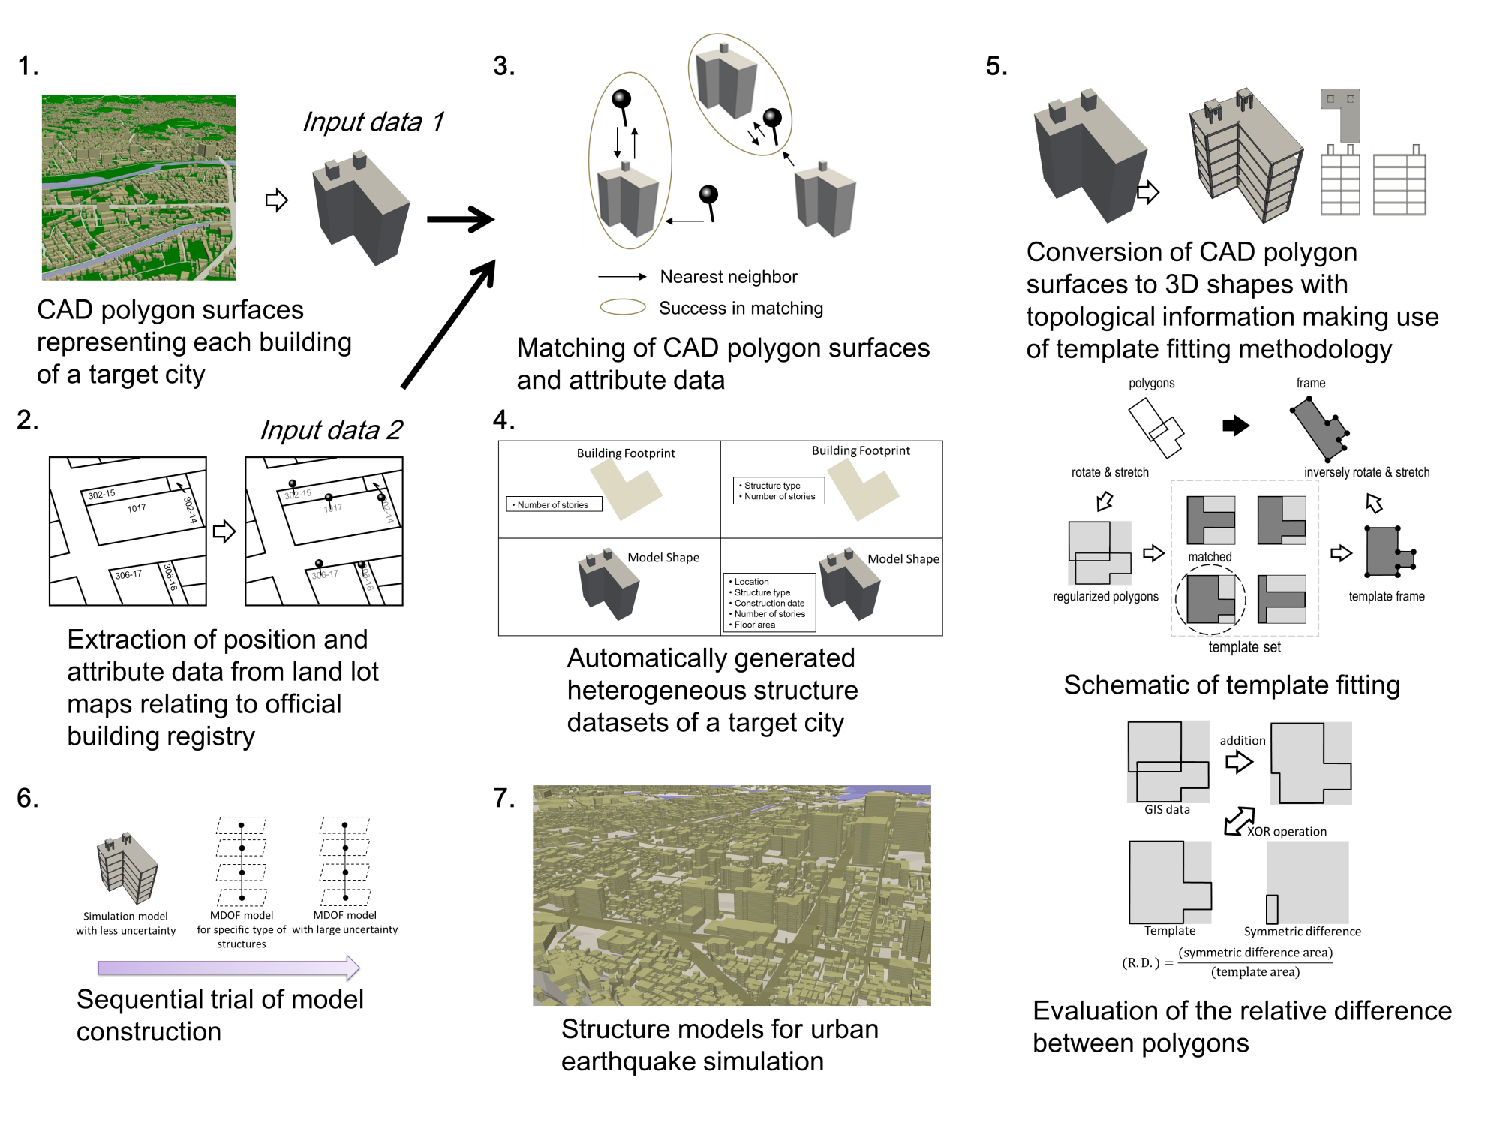
\includegraphics[scale=0.5]{research/hori/figure/platform.pdf}
\caption{Platform of processing data resources to generate urban area model}
\locallabel{hori:fig:platform}
\end{figure}
%.....................................................................

\subsection{Development of system for liquefaction occurrence estimation}

Liquefaction is occurred through complicated processes of soil and underground water which are influenced by non-linear mechanical properties of soil, permeability of soil, and underground water pressure. When the coupling of soil deformation and underground water flow increases underground water pressure locally, liquefaction is induced. Hence, the liquefaction occurrence ought to be estimated by using simple empirical equations for a large urban area. The equations use engineering indices of soil layers of a target site which are obtained by analyzing boring hole data.

Computational Disaster Mitigation and Reduction Research Unit constructs a system that estimates the liquefaction occurrence by using numerical simulation of the complicated processes of liquefaction. The simulation uses a model of a target site which consists of a few soil layers and underground water. The coupling of soil deformation and underground water flow for a given ground motion is computed by using a non-linear finite element method; see Fig.~\localref{hori:fig:liquefaction}. The non-linear analysis of soil deformation is essential, and the finite element method specially tuned for this non-linear analysis is implemented in K computer

The developed system has two key features. First, the system is able to automatically generate an underground model of soil and underground water. There are a set of boding hole data for 10,000 sites in Kobe City, and the system succeeds to construct the model for all the site. Second, the system is able to simultaneously carry out numerical simulation of the liquefaction occurrence for all the sites. Each site is analyzed independently from each other, even though the same input ground motion, measured or presumed, is used. Suitable parallel I/O is implemented into the system.

%.....................................................................
\begin{figure}
\centering
\includegraphics[scale=0.5]{research/hori/figure/liquefaction.eps}
\caption{System of liquefaction occurrence estimation}
\locallabel{hori:fig:liquefaction}
\end{figure}
%.....................................................................

%.....................................................................
\subsection{Estimation of lifeline damage induced by earthquake}

Lifeline is a dense network of pipelines that carry energy (electricity and gas), water and sewage, and communication, in an urban area. The pipelines are mostly buried, and, in general, has higher seismic safety compared with structures on the ground. However, the lifeline plays a fundamental role of supporting various activities in an urban area, and a damage of one spot could induce mal-functioning of a certain portion of the network.

A buried pipeline of the lifeline is damaged by ground deformation which is quantified in terms of strain; structures on the ground is damaged by ground motion which is quantified in terms of acceleration or velocity. Hence, three-dimensional analysis of underground structure responses is essential to estimate lifeline damage induced by an earthquake. Moreover, there is no device which measures ground deformation; it is possible to compute ground strain by distributing seismographs, but measuring strain along the pipeline remains a difficult task for the distributed seismographs. The numerical simulation of ground deformation is a unique solution for the estimate lifeline damage.

Using a largest scale finite element method that is implemented in K computer, Computational Disaster Mitigation and Reduction Research Unit is developing a system that estimate lifeline damage of an urban area of a few kilo meter. Numerically simulating ground deformation in this area is used to estimate candidates of the lifeline damage induced by ground motion; see Fig.~\localref{hori:fig:ground_deformation}.

While natural frequency of man-made structure is in the range of a few Hz, it is a standard practice to measure and analyze seismic response in this temporal resolution. A buried pipeline, however, is not damaged by being shaken but by being pulled or pushed, which could be a faster phenomenon than vibration. We thus need to collaborate with experiments in which failure of buried pipeline induced by ground motion is observed.

%.....................................................................
\begin{figure}
\centering
\includegraphics[scale=0.5]{research/hori/figure/ground_deformation.eps}
\caption{Example of ground deformation distribution and induced lifeline damage}
\locallabel{hori:fig:ground_deformation}
\end{figure}
%.....................................................................

\section{Schedule and Future Plan}

The fiscal year of 2016 is the final year of the first phase of the unit; the extension of the unit is determined. We plan to make a next-generation hazard map for a few cities in Hyogo Prefecture, using the system that processes available data resources. Collecting such data is essential, since the system is completed; sustainable improvement is made for the system. Collaboration of regional universities is strengthened, especially one with University of Hyogo. We also plan to combine tsunami simulation to ground motion simulation.

The objectives of the unit research are summarized as follows: 1) Construction of next generation urban area model for a few cities in Hyogo Prefectures; 2) development of system for liquefaction occurrence estimation; and 3) smart visualization of numerical simulation results of earthquake hazard and disaster.

%%% DO NOT EDIT BELOW

\section{Publications}

%\printbibliography[keyword=journal, heading=subbibliography, title={Journal Articles}, prefixnumbers={1-}, resetnumbers=true]
%\printbibliography[keyword=proceedings, heading=subbibliography, title={Conference Papers}, prefixnumbers={2-}, resetnumbers=true]
%\printbibliography[keyword=invited, heading=subbibliography, title={Invited Talks}, prefixnumbers={3-}, resetnumbers=true]
%\printbibliography[keyword=poster, heading=subbibliography, title={Posters and Presentations}, prefixnumbers={4-}, resetnumbers=true]
%\printbibliography[keyword=deliverable, heading=subbibliography, title={Patents and Deliverables}, prefixnumbers={5-}, resetnumbers=true]

\printbibliography[keyword=journal, heading=subbibliography, title={Journal Articles}, resetnumbers=true]
\printbibliography[keyword=proceedings, heading=subbibliography, title={Conference Papers}]
\printbibliography[keyword=invited, heading=subbibliography, title={Invited Talks}]
\printbibliography[keyword=poster, heading=subbibliography, title={Posters and Presentations}]
\printbibliography[keyword=deliverable, heading=subbibliography, title={Patents and Deliverables}]

\end{refsection}
